\section{Fixed-diffusion similarity and the force-flat cascade space}
\label{im:section}

The finite third-return theorem supplies one positive interval of equal
thermal diffusivity and viscosity.  This section proves that the interval
does not shrink merely because a finite packet is placed at a smaller
physical scale.  The exact Boussinesq similarity transfers any one value
in that interval to any prescribed positive physical diffusion.

The same map also identifies the next infinite-stage defect.  A raw
sequence of rescaled copies has force jets which diverge at exact powers
of the spatial radius.  This obstruction defines the weighted
force-flat space that a corrected sequence must occupy.  The definition
retains the scalar force, the vector force, every space-time derivative,
the physical diffusion, and the full finite return.  It is not an
assertion that the required corrected packet sequence has already been
constructed.

\subsection{Exact two-parameter similarity with both forces retained}

Let $(\widetilde\theta,\widetilde u,\widetilde p,
\widetilde f_\theta,\widetilde f_u)$ be smooth on
$\mathbb R^2_y\times[0,\widetilde T]$ and solve
\begin{align}
 \partial_\tau\widetilde\theta+
 \widetilde u\cdot\nabla_y\widetilde\theta
 &=\delta\Delta_y\widetilde\theta+\widetilde f_\theta,
 \label{im:normalized-scalar}\\
 \partial_\tau\widetilde u+
 (\widetilde u\cdot\nabla_y)\widetilde u+\nabla_y\widetilde p
 &=\delta\Delta_y\widetilde u+\widetilde\theta e_2+
   \widetilde f_u,\qquad
 \operatorname{div}_y\widetilde u=0 .
 \label{im:normalized-vector}
\end{align}
No coefficient in these equations is normalized away: $\delta\geq0$
is the common dimensionless diffusion.

Fix $r,c>0$, a spatial centre $x_*$, and a starting time $t_*$.  Put
\begin{equation}\label{im:variables}
 y=\frac{x-x_*}{r},\qquad
 \tau=\frac{t-t_*}{c},
\end{equation}
and define
\begin{align}
 \theta(x,t)&=\frac{r}{c^2}\widetilde\theta(y,\tau),&
 u(x,t)&=\frac{r}{c}\widetilde u(y,\tau),&
 p(x,t)&=\frac{r^2}{c^2}\widetilde p(y,\tau),
 \label{im:field-map}\\
 f_\theta(x,t)&=\frac{r}{c^3}\widetilde f_\theta(y,\tau),&
 f_u(x,t)&=\frac{r}{c^2}\widetilde f_u(y,\tau),&
 d&=\frac{r^2}{c}\delta .
 \label{im:force-map}
\end{align}

\begin{proposition}\label{im:similarity}
The tuple in \eqref{im:field-map}--\eqref{im:force-map} solves the same
Boussinesq system on
$\mathbb R^2_x\times[t_*,t_*+c\widetilde T]$ with equal physical
diffusion $d$.  The map is invertible.  Spatial supports are translated
by $x_*$ and multiplied by $r$; time intervals are multiplied by $c$.
The vorticity obeys
\begin{equation}\label{im:vorticity-scale}
 \omega(x,t)=\frac1c\widetilde\omega(y,\tau).
\end{equation}
\end{proposition}

\begin{proof}
Every term is kept.  The scalar terms are
\[
 \partial_t\theta=\frac r{c^3}\partial_\tau\widetilde\theta,\qquad
 u\cdot\nabla_x\theta
 =\frac r{c^3}\widetilde u\cdot\nabla_y\widetilde\theta,\qquad
 d\Delta_x\theta
 =\frac{d}{rc^2}\Delta_y\widetilde\theta
 =\frac r{c^3}\delta\Delta_y\widetilde\theta.
\]
For momentum,
\[
 \partial_tu=\frac r{c^2}\partial_\tau\widetilde u,\quad
 (u\cdot\nabla_x)u=\frac r{c^2}
       (\widetilde u\cdot\nabla_y)\widetilde u,\quad
 \nabla_xp=\frac r{c^2}\nabla_y\widetilde p,
\]
while
\[
 d\Delta_xu=\frac d{rc}\Delta_y\widetilde u
 =\frac r{c^2}\delta\Delta_y\widetilde u,\qquad
 \theta e_2=\frac r{c^2}\widetilde\theta e_2.
\]
Thus the scalar equation has common factor $r/c^3$ and the vector
equation has common factor $r/c^2$.  Also
$\operatorname{div}_xu=c^{-1}\operatorname{div}_y\widetilde u$.
All scale factors are positive, so reversing
\eqref{im:variables} and reciprocating the factors gives the inverse.
One spatial derivative of $u$ proves \eqref{im:vorticity-scale}.
The support and interval assertions follow directly from the affine
coordinate map.
\end{proof}

\subsection{The finite return at arbitrary physical diffusion and scale}

Choose once and for all
\begin{equation}\label{im:delta-star}
 0<\delta_*\leq d_{\rm ret},
\end{equation}
where $d_{\rm ret}$ is the positive number constructed in
Theorem~\ref{trc:third-return}.  For any prescribed physical diffusion
$d>0$ and any $r>0$, set
\begin{equation}\label{im:parabolic-clock}
 c(r;d,\delta_*)=\frac{\delta_*}{d}r^2.
\end{equation}
Then $dc/r^2=\delta_*$ exactly.

The controls and amplitudes carried by the finite packet transform with
the fields.  If a tilde denotes the packet before similarity, then
\begin{equation}\label{im:control-map}
 \alpha(t)=\widetilde\alpha(\tau),\qquad
 K_j=r^{-1}\widetilde K_j,\qquad
 \Theta_j(t)=\frac r{c^2}\widetilde\Theta_j(\tau),\qquad
 \Omega_j(t)=\frac1c\widetilde\Omega_j(\tau),\qquad
 \sigma_j=\frac1c\widetilde\sigma_j .
\end{equation}
Indeed $K_j\Theta_j$ is a temperature-gradient amplitude and therefore
has factor $c^{-2}$, while $\Omega_j$, $\dot\alpha$, and $\sigma_j$ are
vorticity-scale quantities and therefore have factor $c^{-1}$.

\begin{theorem}\label{im:fixed-d-return}
For every $d>0$ and $r>0$, the similarity image of the complete finite
third-return solution at diffusion $\delta_*$ is a complete finite
third-return solution at physical diffusion $d$, supported at spatial
scale $r$ and running for
$c(r;d,\delta_*)\widetilde T$.  It retains
\[
 Z(T)=0,\qquad \Omega_3(T)=0,\qquad\Theta_3(T)<0,
\]
and the dimensionless endpoint bounds
\[
 \frac{\Omega_2(T)}{\sigma_2}\geq\frac1{48},\qquad
 \log\frac{-\Theta_3(T)}{-\Theta_3(0)}\geq\frac1{24},\qquad
 \frac{2\dot\alpha(T)+\Omega_1(T)+\Omega_2(T)}{\sigma_2}
 \geq\frac{c_W}{4}.
\]
Thus fixed positive diffusion creates no new finite-stage scale
restriction after parabolic similarity.
\end{theorem}

\begin{proof}
Apply Proposition~\ref{im:similarity} with
$c=\delta_*r^2/d$.  The normalized solution exists and returns by
Theorem~\ref{trc:third-return}.  Positive scale factors preserve all
zeroes and signs.  The first four identities in \eqref{im:control-map}
give the zero, sign, and temperature-ratio assertions.  Every vorticity
and $\dot\alpha$ is multiplied by $c^{-1}$ by
\eqref{im:vorticity-scale} and \eqref{im:control-map}.  The complete
temperature-gradient vector is multiplied by $c^{-2}$; hence each
growth scale $\sigma_j$, defined as the positive square root of its
magnitude, is multiplied by $c^{-1}$.  The two normalized vorticity
bounds are therefore unchanged.  Supports and duration follow from the
same similarity map.
\end{proof}

This is stronger than a stagewise choice of ever smaller physical
diffusion.  One fixed $d>0$ works at every radius.  The cost appears in
the amplitudes and forces, which the next calculation makes exact.

\subsection{Every field and force jet}

Let $\gamma\in\mathbb N_0^2$ and $b\in\mathbb N_0$.  Direct
differentiation of \eqref{im:field-map}--\eqref{im:force-map} gives
\begin{align}
 \partial_x^\gamma\partial_t^b u
 &=r^{1-|\gamma|}c^{-1-b}
   (\partial_y^\gamma\partial_\tau^b\widetilde u)(y,\tau),
 \label{im:u-jets}\\
 \partial_x^\gamma\partial_t^b \theta
 &=r^{1-|\gamma|}c^{-2-b}
   (\partial_y^\gamma\partial_\tau^b\widetilde\theta)(y,\tau),
 \label{im:theta-jets}\\
 \partial_x^\gamma\partial_t^b p
 &=r^{2-|\gamma|}c^{-2-b}
   (\partial_y^\gamma\partial_\tau^b\widetilde p)(y,\tau),
 \label{im:p-jets}\\
 \partial_x^\gamma\partial_t^b f_u
 &=r^{1-|\gamma|}c^{-2-b}
   (\partial_y^\gamma\partial_\tau^b\widetilde f_u)(y,\tau),
 \label{im:fu-jets}\\
 \partial_x^\gamma\partial_t^b f_\theta
 &=r^{1-|\gamma|}c^{-3-b}
   (\partial_y^\gamma\partial_\tau^b\widetilde f_\theta)(y,\tau).
 \label{im:ftheta-jets}
\end{align}
At the fixed-diffusion clock \eqref{im:parabolic-clock}, these factors
are respectively
\begin{align}
 &(d/\delta_*)^{1+b}r^{-1-|\gamma|-2b},
 &&(d/\delta_*)^{2+b}r^{-3-|\gamma|-2b},
 \label{im:state-powers}\\
 &(d/\delta_*)^{2+b}r^{-2-|\gamma|-2b},
 &&(d/\delta_*)^{2+b}r^{-3-|\gamma|-2b},
 \nonumber\\
 &(d/\delta_*)^{3+b}r^{-5-|\gamma|-2b}.
 \label{im:force-powers}
\end{align}
The first row contains the velocity and scalar factors; the second row
contains pressure, vector force, and scalar force in that order.
Every power of $r,d,\delta_*$ is retained.

\subsection{Why raw repeated packets fail}

The complete finite packet has a nonzero normalized vector force.  During
its initial interpolation the base velocity is zero and
$\dot\alpha=0$.  Equations \eqref{eq:basephysical} and
\eqref{eq:baseforces} give
\[
 \widetilde f_u=-\widetilde\theta_b e_2.
\]
The retained initial temperature is nonzero, so there is a normalized
space-time point $(y_\dagger,\tau_\dagger)$ and a number $a_\dagger>0$
with
\begin{equation}\label{im:nonzero-force}
 |\widetilde f_u(y_\dagger,\tau_\dagger)|=a_\dagger.
\end{equation}

\begin{proposition}\label{im:raw-obstruction}
Let $r_q\downarrow0$, let $t_q\to T_*$, and place complete similarity
copies with the fixed clock
$c_q=\delta_*r_q^2/d$ at the common spatial centre $x_*$.  At the
corresponding points
\[
 x_q=x_*+r_qy_\dagger,\qquad
 s_q=t_q+c_q\tau_\dagger,
\]
one has
\begin{equation}\label{im:raw-blowup}
 |f_{u,q}(x_q,s_q)|
 =a_\dagger(d/\delta_*)^2r_q^{-3}\longrightarrow\infty.
\end{equation}
Consequently $f_{u,q}$ does not tend to zero locally uniformly near
$(x_*,T_*)$.  The series $\sum_qf_{u,q}$ therefore cannot converge
uniformly on any compact neighborhood of that point, because uniform
convergence of a function series requires its terms to tend uniformly
to zero.  Repeating the finite return without a force-flattening
correction therefore fails the packet-series convergence required by
the infinite construction.
\end{proposition}

\begin{proof}
The points converge to $(x_*,T_*)$ because $r_q,c_q\to0$.
Insert \eqref{im:nonzero-force} into \eqref{im:fu-jets} with
$b=|\gamma|=0$, then use \eqref{im:parabolic-clock}.  This is exactly
\eqref{im:raw-blowup}.  Fix a compact neighborhood $K$ of
$(x_*,T_*)$.  For every sufficiently large $q$, $(x_q,s_q)\in K$, and
therefore
\[
 \sup_K|f_{u,q}|\geq
 a_\dagger(d/\delta_*)^2r_q^{-3}\longrightarrow\infty.
\]
If the series of forces converged uniformly on $K$, the differences of
successive partial sums, namely $f_{u,q}$, would converge uniformly to
zero.  The displayed lower bound rules this out.
\end{proof}

This obstruction is distinct from the unchanged-state Laplacian
obstruction in Section~\ref{sec:infinitecost}.  The similarity map
absorbs the physical diffusion into each finite packet; the new defect
is the scale of the packet's remaining force.

\subsection{The force-flat space defined by the obstruction}

For a sequence of normalized corrected packets, write
\begin{align}
 \varepsilon^u_{q,b,\gamma}
 &=\sup|\partial_y^\gamma\partial_\tau^b
                \widetilde f_{u,q}|,&
 \varepsilon^\theta_{q,b,\gamma}
 &=\sup|\partial_y^\gamma\partial_\tau^b
                \widetilde f_{\theta,q}|.
 \label{im:normalized-budgets}
\end{align}
The supremum is taken on the full normalized support and time interval;
no phase, cutoff, pressure, or joining region is omitted.

\paragraph{Definition (the force-flat packet space).}\label{im:force-flat-definition}
At physical diffusion $d$ and normalized diffusion $\delta_*$, the
force-flat packet space $\mathfrak F(d,\delta_*)$ consists of sequences
$(r_q,\widetilde f_{\theta,q},\widetilde f_{u,q})$ with $r_q\downarrow0$
and normalized forces in
$C_c^\infty(\mathbb R^2\times\mathbb R)$ such that, for every
$m\in\mathbb N_0$,
\begin{align}
 \sum_q\ \max_{b+|\gamma|\leq m}
 &(d/\delta_*)^{2+b}
 r_q^{-3-|\gamma|-2b}\varepsilon^u_{q,b,\gamma}<\infty,
 \label{im:flat-u}\\
 \sum_q\ \max_{b+|\gamma|\leq m}
 &(d/\delta_*)^{3+b}
 r_q^{-5-|\gamma|-2b}\varepsilon^\theta_{q,b,\gamma}<\infty.
 \label{im:flat-theta}
\end{align}

These are the complete force weights imposed by the PDE similarity,
not chosen regularity exponents.  Translate and rescale each compactly
supported force by \eqref{im:variables}--\eqref{im:force-map}, and extend
it by zero.  Then \eqref{im:flat-u}--\eqref{im:flat-theta} give uniform
convergence of every derivative on compact sets by the Weierstrass test.
The fundamental theorem of calculus in each coordinate identifies the
limits of the derivative series with the derivatives of the force
limit.  Hence the force sum is smooth.  Spatial and temporal support,
state convergence, nonlinear residual convergence, endpoint matching,
and the blowup property remain additional equations of the construction;
the force-flat definition does not conceal them.

The weight space has nonzero elements.  Choose fixed nonzero functions
$\Phi_u\in C_c^\infty(\mathbb R^2\times(0,1);\mathbb R^2)$ and
$\Phi_\theta\in C_c^\infty(\mathbb R^2\times(0,1))$, and set
\begin{equation}\label{im:explicit-budget}
 r_q=2^{-q},\qquad
 \widetilde f_{u,q}=2^{-q^2}\Phi_u,\qquad
 \widetilde f_{\theta,q}=2^{-q^2}\Phi_\theta
 \quad(q\geq1).
\end{equation}
For each fixed derivative pair, the corresponding quantities in
\eqref{im:normalized-budgets} equal $2^{-q^2}$ times the finite
derivative supremum of $\Phi_u$ or $\Phi_\theta$.  The maximum of these
finitely many profile constants for $b+|\gamma|\leq m$ is a finite
number $C_m$ independent of $q$.
For $b+|\gamma|\leq m$, the worst vector-force radius power is
$r_q^{-3-2m}$ and the worst scalar-force radius power is
$r_q^{-5-2m}$.  Thus their variable parts are bounded by
\[
 2^{-q^2+(3+2m)q},\qquad
 2^{-q^2+(5+2m)q}.
\]
The successive-term ratios are
\[
 2^{-2q+2m+2},\qquad 2^{-2q+2m+4}.
\]
They are at most $1/2$ for all $q\geq m+2$ and $q\geq m+3$,
respectively.  Multiplication by $C_m$ and the fixed powers of
$d/\delta_*$ does not affect convergence.  Both series converge for
every fixed $m$.  This constructs nonzero elements with a simultaneous
superalgebraic budget for every force jet.

\subsection{First realization attempt and the exact next calculation}

The raw finite packet has
$\varepsilon^u_{q,0,0}\geq a_\dagger$, so
Proposition~\ref{im:raw-obstruction} proves that it does not belong to
$\mathfrak F(d,\delta_*)$.  The direct unchanged-state force repair also
does not belong: Section~\ref{sec:infinitecost} gives its stronger
pointwise scalar, vector, and curl divergences.  The current finite
source-chart estimates do not repair this.  They contain negative powers
of the chart parameter and no sequence of normalized residual gains
$\varepsilon_{q,b,\gamma}$.

The calculation nevertheless changes the infinite problem in two exact
ways.  First, fixed positive diffusion is compatible with every finite
return scale through \eqref{im:parabolic-clock}.  This removes the
isolated packet's scale restriction; it does not prove a diffusion
bound uniform for the coupled infinite sequence.  Second, the target of
the correction cycle is now explicit:
after all pressure, mean, cutoff, old-wave, quadratic, evaluated-phase,
and joining terms have been assembled, its normalized force jets must
land in \eqref{im:flat-u}--\eqref{im:flat-theta}.  The concrete budget
\eqref{im:explicit-budget} shows the amount of decay which suffices.

The next construction step is therefore to retain the returned parent,
calculate the type-compatible Boussinesq increment residual, and construct
an actual correction of that residual.  The separate three-dimensional
Navier--Stokes moment and stress operations cannot be applied here without
first proving their receiving map for these scalar and vector fields.
The based residual and state map are derived in Section~\ref{ibc:section};
the first compact local correction is constructed in
Section~\ref{irc:section}.  The remaining all-stage calculation must put
every actual force jet of order at most $q$ below $2^{-q^2}$ and prove
the complete next-stage state match.

The similarity identities, radius exponents, and ratio tests in this
section are checked independently by
\texttt{infinite\_modified/checks/parabolic\_similarity\_check.py}.
Figure~\ref{im:fig:similarity} displays the exact finite-to-infinite
separation.

\begin{figure}[htbp]
 \centering
 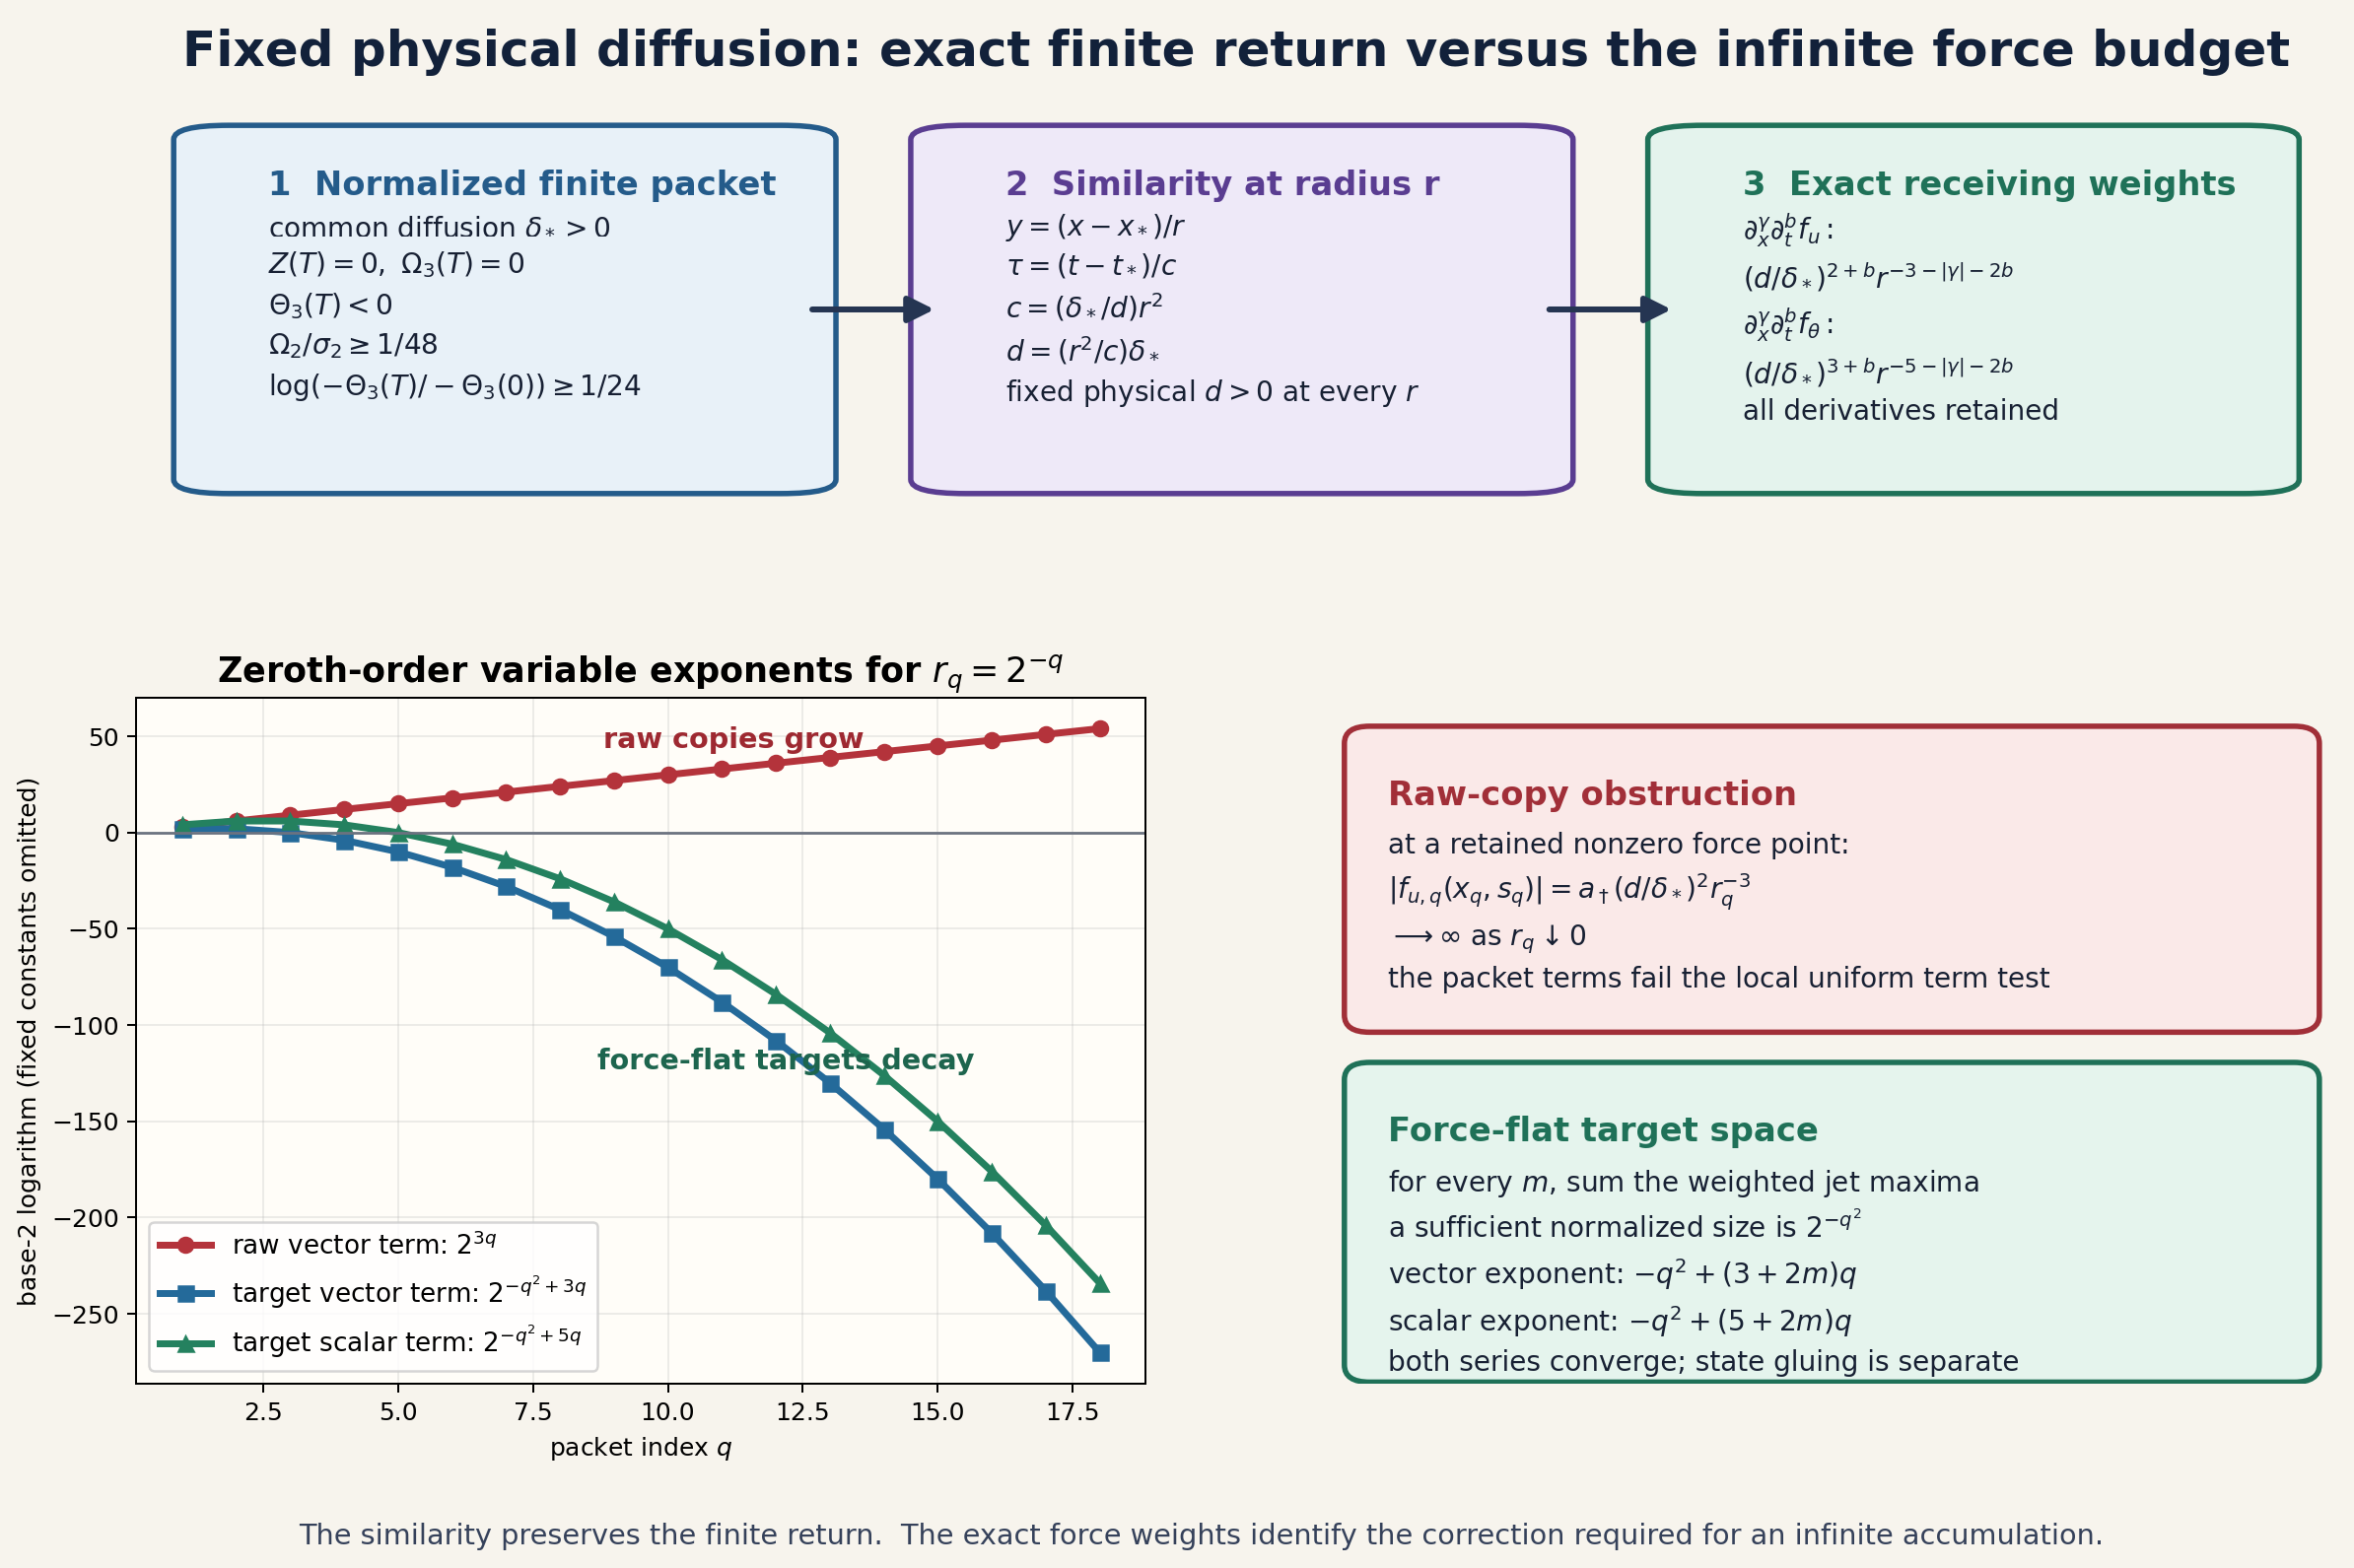
\includegraphics[width=0.96\linewidth]
 {infinite_modified/figures/fixed_diffusion_similarity.png}
 \caption{The fixed-diffusion similarity window.  Parabolic scaling
 transfers the complete finite return to every radius, while the exact
 force-jet powers show that raw copies fail the local uniform term test.
 The force-flat weights are the receiving space for the still-required
 correction and gluing operations.}
 \label{im:fig:similarity}
\end{figure}
